\documentclass[11pt,a4paper,titlepage]{article}

%\usepackage{pdflscape}
\usepackage[margin=1in]{geometry}
\usepackage{titling}
%\usepackage{graphicx}
\usepackage[hidelinks]{hyperref}
\usepackage{graphicx}
\usepackage{float}

\newcommand{\subtitle}[1]{%
  \posttitle{%
    \par\end{center}
    \begin{center}\large#1\end{center}
    \vskip0.5em}%
}

\begin{document}
\title{Software Requirements Specification and Technology Neutral Process Design}
\subtitle{ Git: \url{https://github.com/FrikkieSnyman/COS301_GroupProject}}

\DeclareGraphicsExtensions{.png}
\graphicspath{{../drawings/}}

\author{\textbf{COS301 Main Project - The fellowship of the CIN}\\
Frikkie Snyman 13028741\\
Hanrich Potgieter stdnt num\\
Hugo Greyvenstein 13019989\\
Andre Calitz 13020006\\
Chris Cloete 13029721\\}

\maketitle1

\tableofcontents
\pagebreak

\setlength{\parindent}{0em}
\setlength{\parskip}{0.5em}
\section{Introduction}
%just use \input{file} here
	The aim of this document is to provide the reader with sufficient insight into the system at hand, so that the system can be maintained and developed by a third-party without further input needed. The initial development of this system made use of agile software development, and thus, not all specifications, as provided by the client, is known beforehand. The client, however will form an integral part in the constant development of this system due to the aforementioned reasons. This document, acts as an initial impression of the Architectural and Functional requirements for the project at hand.

\section{Vision}
	The client, being EpiUse Advance, requests for an application to be produced to assist in estimating the time frame and complexity of tasks presented to the client for development. The project at hand will form as a platform for experts to anonymously produce estimations, with a certain level of confidence for these tasks. For each task, a project manager of sorts can then view the estimations, and based on these estimations determine if there is misunderstanding between developers and/or experts in the team. Further statistical analysis can be performed on the estimations, to include graphs.

\section{Background}
 	The biggest reason leading to this project, is that EpiUse Advance is having trouble providing a quote to their potential clients with confidence. Oftentimes, it would happen that EpiUse Advance would have difficulty specifying to their clients the costs involved in developing their proposed tasks. This project aims to relieve this issue from EpiUse Advance.
\newpage 
\section{Software and Architecture Requirements}
	% \input{Architectural_Requirements/architecturesAndFrameworks.tex}
	
	\subsection{Access and Integration requirements}
\subsubsection{Access Channels}
\begin{itemize}
	\item{Human Access Channels}\newline\newline
	The system will primarily be accessed via a web browser, which should then be able to access the services offered by the 	system through RESTful web services. Furthermore, the system will be written in such a way to easily produce a mobile app, thus allowing users to also access the same system via a mobile application.
\end{itemize}
\subsubsection{Integration Channels}
\begin{itemize}
\item{LDAP}\newline\newline
The system needs to integrate with an existing user database as provided by EpiUse Advance. The system will make use of LDAP in order to achieve this, since the existing database is already set up with this protocol.
\end{itemize}

	\subsection{Architectural Responsibilities}
The system will have to log estimations being made by various users. The system must also be able to keep a history of these estimations. Furthermore, the system must be able to store projects and/or their associated tasks. Hence, the system must persist these projects to a database, along with persisting the estimations being made associated by the project and user making them. \\ \\
The system will make use of Node Package Manager, which automatically provides an execution environment for the system.
	\subsection{Quality Requirements}
\subsubsection{Critical}
{\bfseries Functionality:} The functionality the system will provide is very important since the estimations given by different experts need to be analysed and visualized in some way for a human user to easily make a decision. The users of the system will access the functionality of the system to aid them in the development of products for clients by providing the human user with visualisations of data, to enable them to make more accurate and informed estimations. The more functionality provided for data-analysis the more successful the project will be regarded.
\\ \\
{\bfseries Pluggability:} The client plans on expanding the system if it is successfully deployed within the company and the system improves their experience with regards to making estimations for internal projects. The client should have the ability to develop plug-ins to expand the functionality of the system e.g. artificial intelligence, more parameters for estimation, more detailed creation of project tree etc.
\\ \\
{\bfseries Usability:} Usability is important since the process of making estimations should not be cumbersome and frustrating for the users. The system is meant to improve the process of making estimations and user experience is very important to ensure that users give the correct-, honest estimations without rushing the process, because it's tedious, and possibly affecting the outcome of the estimation decisions.

\subsubsection{Important}
{\bfseries Maintainability:} The maintainability of the system should be kept in mind while developing the system, because the client will be using the system for everyday operations of the company and the system's availability should be ensured by making it sufficiently maintainable.
\\ \\
{\bfseries Scalability:} The client does not require the system to be used by a large amount of people at the same time. According to the requirements of the client at most ten people will be making estimations at the same time, but because we plan on making the system open-source scalability should be kept in mind such that the system will be somewhat scalable.

\subsubsection{Nice to have}
\begin{itemize}
	\item{Security}
	\item{Performance}
	\item{Reliability}
\end{itemize}

	\subsection{Architectural Constraints}
The client has requested to make use of the following protocol:
\begin{itemize}
	\item LDAP
	\\ \\
	LDAP must be used to allow the system to integrate with the existing user database as provided by the client.
\end{itemize}
	% \input{Architectural_Requirements/architecturesAndFrameworks.tex}
	\subsection{Technologies}
The following technologies will be used in the implementation of the system:\\ \\
{\bfseries Client Side:}
\begin{itemize}
	\item AngularJS: \\ \\
	AngularJS is a technology used on the client side to make it possible to server dynamic view in web-applications. This technology is also fully extensible, thus allowing it to work well with any other libraries.
	\item Bootstrap: \\ \\
	Bootstrap is an HTML, CSS and JavaScript framework. Making use of Bootstrap allows for easy development of responsive projects, allowing the web-application to look beautiful on almost any platform.
	\item jQuery: \\ \\
	jQuery is a very powerful JavaScript library, which makes things like animations, document manipulation,AJAX, etc. so much simpler to handle. jQuery is an API that works across multiple browsers, allowing compatibility over multiple platforms
	\item D3: \\ \\
	D3 is a JavaScript library which is used to manipulate documents which is based on data. D3 is used to visually represent the data contained within the document.
\end{itemize}

{\bfseries Server Side:}
\begin{itemize}
	\item Node.js:\\ \\ 
	Node.js is an API which is used to easily build scalable, and fast network applications. The API is inherently asynchronous to increase server-side performance.
	\item Node Package Manager:\\ \\
	Node Package Manager is used by node.js to manage the packages which will be used on the server. This allows a uniform execution environment to exist.
	\item MongoDB: \\ \\
	MongoDB is a document database based on the NoSQL movement. It allows to be very agile, whilst still maintaining scalability and performance.
	\item mongoose \\ \\
	Mongoose will provide us with connection to the database. Schemers will provide us with consistent data in the database.
	\item ldapjs \\ \\
	This will allow us to connect to the client database and obtain the user data.
\end{itemize}
{\bfseries Mobile Application}
\begin{itemize}
	\item PhoneGap:\\ \\
	PhoneGap is a utility that creates mobile application from web based technologies. This utility integrates nicely with all the aforementioned technologies in order to produce a mobile, responsive application for smartphones.
\end{itemize}
{\bfseries Testing and Integration}
\begin{itemize}
	\item Nodeunit:\\ \\
	Nodeunit will be used to write unit tests for the server side node modules.
	\item Jasmine and Karma:\\ \\
	These technologies will be used to perform tests on behavioral JavaScript, as written with the use of AngularJS.
	\item Travis CI:\\ \\
	Travis CI will be used to integrate functions based on their appropriate unit tests.
\end{itemize}
	\subsection{Architectural Patterns}
\subsubsection{Model-View-Controller}
We will use the MVC pattern to implement the user interface.
\begin{itemize}
	\item{Model}
	\newline
	The model will be implemented by making use of Express.js
	\item{View}
	\newline
	The view will be implemented using Bootstrap.
	\item{Controller}
	\newline
	The controller will be implemented by using Angular.js
	\begin{figure}[H]
	    	\centering
	    	\fbox{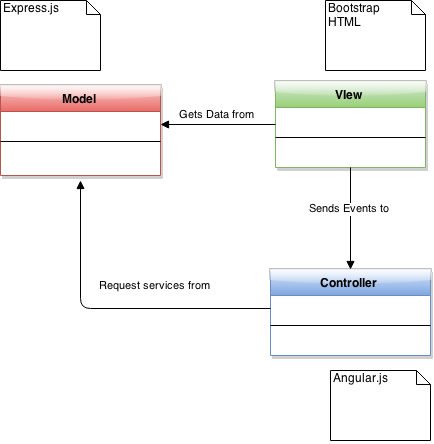
\includegraphics[width=0.5\textwidth]{MVC}}
	    	\caption{Model View Controller}
	    	\label{fig:Learning rate 0.1}
   	\end{figure}
\end{itemize}
	\subsection{Architectural Tactics}
\subsubsection{Minimize Technology suite}
	A minimal suite of technologies will be used to improve the maintainability of the system as well as minimize the complexity of the system and reduce the chance of interference of between technologies.
\subsubsection{Contracts Based Development}
	Contracts will be enforced across services as well as data structure constraints. This is done to improve flexibility and testability of the system.
\subsubsection{Support Plug-in Framework}
	A plug-in framework will be provided to facilitate flexibility. This will allow addition functionality to easily be added into the system
\subsubsection{Database Abstraction}
	The system will provide a database abstraction layer to improve the flexibility and deployability.
\subsubsection{Automated Persistence Mapping}
	Automated persistence mapping will be used simplify the replacement of persistence technologies, reduce code bulk and also to avoid polluting application logic with persistence logic.
\subsubsection{Caching}
	Caching of resources will be used to address scalability.
\subsubsection{Connection pooling}
	Database connection pooling will be used to address scalability by reusing resources.
\subsubsection{Templating}
	Templates will be used to address usability by providing a consistent UI, this will also address maintainability.
\subsubsection{UI Components Framework}
	The system will make use of rich dynamic JavaScript libraries in order to provide improved the usability of the system as well as address maintainability and scalability by reusing components.
\subsubsection{Asynchronous Processing}
	To address scalability the system will make use of asynchronous processing to avoid having to wait for for certain non-critical time consuming tasks to be completed whilst other more important requests are being made.
\subsubsection{Off-load Rendering Responsibilities to Client}
	Rendering of pages will be handled on the client side to improve the usability as well scalability of the system.
\subsubsection{REST Web-services}
	To address integrability RESTful web services will be employed in the system, with the request and result objects encoded in JSON. This will allow for easier development of multiple clients as well as allow other systems to use the provided services.
\subsubsection{Logging}
	Logging will be used to capture audit data for the system.
\newpage
% \input{AccessChannels/AccessChannels.tex}%leave it alone, my headings are in the file
\newpage
\section{Functional Requirements and application design}
	\subsection{User Management}
This module is responsible for reading data from the client user database. It will do this by making use of ldap.js .
\subsubsection{Scope}
\paragraph{Test}
\subsubsection{Use cases}
\begin{itemize}
\item Autorize
\item validateUserName
\item retrieveEmail
\end{itemize}
\subsubsection{Domain model}

\subsection{Project}
The project module is responsible for the representation and persistence of all projects that the system will use to do the estimations on. This module will allow for complex projects to be created, as well as to be updated. A project is represented as a tree, consisting of a top-level project node and lower-level task nodes.

\subsubsection{Scope}

\subsubsection{Use cases}

\paragraph{Create a project - priority: critical}
Users with sufficient privileges can create projects.

\paragraph{Get project - priority: critical}
Users with sufficient privileges can retrieve projects to view them, or to be used for other purposes. This use case must thus return a representation of the project-tree, and not produce the output of the project tree.

\paragraph{Hide project}
\paragraph{Update project - priority: critical}


\subsubsection{Domain model}
\subsection{Estimation}
\subsubsection{Scope}
\subsubsection{Use cases}
\subsubsection{Domain model}
\subsection{Report}
\subsubsection{Scope}
\subsubsection{Use cases}
\subsubsection{Domain model}
%============================
%Notification
%============================
\subsection{Notification}
This module will be responsible to notify all the users as required by the projects estimation. The estimation module will log a message request to the notification and add all the required users to notify.
\subsubsection{Scope}
This is the notification scope
	\begin{figure}[H]
	    	\centering
	    	\fbox{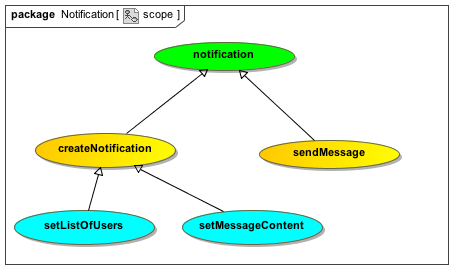
\includegraphics[width=0.8\textwidth]{Notification_Scope}}
	    	\caption{Notifications Scope}
	    	\label{fig:Notification_Scope}
   	\end{figure}
\subsubsection{Use cases}
The main purpose of notifications is to notify users with the required message. The project will supply the list of users to notify and the contents of the message.
\subsubsection{Domain model}

\end{document}
